\chapter{Statistika a BL}

\section{Benford's Law Formulation}



\subsection{Variations of BL} 

In this section we shall use the same terminology as mentioned by \citeauthor{kossovsky2014benford}. 


\subsubsection{First Leading Digits Law FL} 

%První číslice je ta, kterou nalezneme na nejvyšším řádu a je nenulová. Pro číslo 124.857 by to byla 1, pro číslo 0,03958 zase 3. Podle Benfordova zákona první číslice platí že teoretické četnosti odpovídají pravděpodobnosti ze vztahu \ref{BZ-prvni}, to znamená že číslice 1 se vyskytuje na první pozici v čísle s 0,3 pravděpodobností, číslice 2 0,18 a dále to klesá až číslice 9 s pravděpodobností pouze 0,046. %%%%
\begin{figure}[h]
    \centering
    \caption{Theoretical frequencies for the first digit}
    \label{fig:FL}

\pgfplotsset{width=8.5cm,compat=1.18}
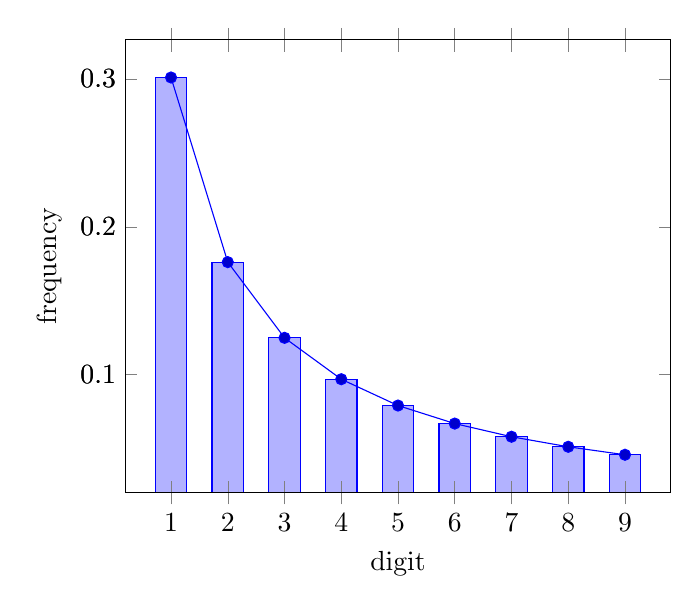
\begin{tikzpicture}
\begin{axis}[
    ybar,
    bar width=.4cm,
    enlargelimits=0.1,
    ylabel={frequency},
    xlabel={digit},
    symbolic x coords={1,2,3,4,5,6,7,8,9},
    xtick=data,
    %nodes near coords,
    %nodes near coords align={vertical},
    ]
\addplot coordinates {(1,0.3010) (2,0.1761) (3, 0.1249) (4,0.0969) (5,0.0791) (6,0.0669) (7,0.0580) (8,0.0512) (9,0.0458)};

\end{axis}

\begin{axis} [
    bar width=.4cm,
    enlargelimits=0.1,
    symbolic x coords={1,2,3,4,5,6,7,8,9},
    xticklabels={},
    xtick=data,
]

    \addplot coordinates {(1,0.3010) (2,0.1761) (3, 0.1249) (4,0.0969) (5,0.0791) (6,0.0669) (7,0.0580) (8,0.0512) (9,0.0458)};
\end{axis}
\end{tikzpicture}
\source{ and processing: author}
\end{figure}

The first digit is the one found at the highest order and is non-zero. In the case of the number 124.857, the first digit would be 1, whereas for the number 0.03958, the first digit would be 3. According to Benford's law of the first digit, the theoretical frequencies correspond to the probabilities from the relation \ref{BZ-first}, indicating that the digit 1 occurs in the first position with a probability of 0.3, the digit 2 with 0.18, and so forth, with the digit 9 occurring with a probability of only 0.046.

\begin{koment}
jak citovat equation?
\end{koment}

\begin{equation}
\label{BZ-first}
\text{P(the digit on the 1st position is the number } d \text{)}= \log_{10}(1+1/d)
\end{equation}



% Pravděpodobnosti pro výskyt daných čísel na první pozici:

% \begin{align*}
% \text{1:} \quad \log_{10}(1+1/1) = \quad 0,3010\\
% \text{2:} \quad \log_{10}(1+1/2) = \quad 0,1761\\
% \text{3:} \quad \log_{10}(1+1/3) = \quad 0,1249\\
% \text{4:} \quad \log_{10}(1+1/4) = \quad 0,0969\\
% \text{5:} \quad \log_{10}(1+1/5) = \quad 0,0791\\
% \text{6:} \quad \log_{10}(1+1/6) = \quad 0,0669\\
% \text{7:} \quad \log_{10}(1+1/7) = \quad 0,0580\\
% \text{8:} \quad \log_{10}(1+1/8) = \quad 0,0512\\
% \text{9:} \quad \log_{10}(1+1/9) = \quad 0,0458
% \end{align*}

%Jak je možné vidět na grafu \ref{fig:first-digit-law}, rozdělení je velmi výrazně zkosené ve prospěch nejnižších číslic. Při posunu na druhou a vyšší číslici se toto zkosení výrazně vyrovná až mezi číslicemi nebude rozdíl 

\begin{koment}
Second Leading Digits    
\end{koment}


The distribution of the second digits is less skewed than that of the first leading digits.

\begin{figure}[h]
    \centering
    \caption{Theoretical frequencies for the 2nd leading digits}  
    \label{fig:second-digit-law}

\pgfplotsset{width=8.5cm,compat=1.18}
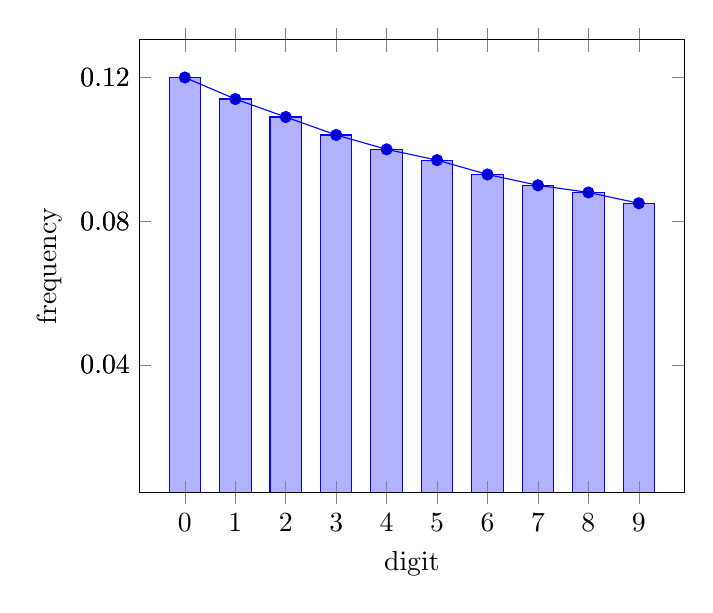
\begin{tikzpicture}
\begin{axis}[
    ybar,
    bar width=.4cm,
    ymin=0.015,
    ytick={0.12, 0.08, 0.04},
    enlargelimits=0.1,
    ylabel={frequency},
    xlabel={digit},
    symbolic x coords={0, 1,2,3,4,5,6,7,8,9},
    xtick=data,
    %nodes near coords,
    %nodes near coords align={vertical},
    yticklabel style={/pgf/number format/fixed, /pgf/number format/precision=2},
    ]
\addplot coordinates {(0,0.12) (1,0.114) (2,0.109) (3, 0.104) (4,0.10) (5,0.097) (6,0.093) (7,0.09) (8,0.088) (9,0.085)};

\end{axis}

\begin{axis} [
    bar width=.4cm,
    ymin=0.015,
    ytick={0.12, 0.08, 0.04},
    enlargelimits=0.1,
    symbolic x coords={0,1,2,3,4,5,6,7,8,9},
    xticklabels={},
    xtick=data,
    yticklabel style={/pgf/number format/fixed, /pgf/number format/precision=2},
]

    \addplot coordinates {(0,0.12) (1,0.114) (2,0.109) (3, 0.104) (4,0.10) (5,0.097) (6,0.093) (7,0.09) (8,0.088) (9,0.085)};
\end{axis}
\end{tikzpicture}
    \source{: \citeauthor{kossovsky2014benford}, \citeyear{kossovsky2014benford}; processing: author}
\end{figure}

As can be seen in the graph \ref{fig:FL}, the distribution is heavily skewed in favour of the lowest digits. As we move to the second (as seen on the graph \ref{fig:second-digit-law}) and higher digits, this skew will flatten out significantly until there is no difference between the digits.  \cite{kossovsky2014benford}

\begin{koment}
    3rd digits are close to being equal, could be worth to add it here too 
\end{koment}

\subsubsection{First Two Leading Digits FTD}

%Modifikací předchozích dvou je pravděpodobnost dvou po sobě jdoucích čísel na první a druhé pozici \ref{BZ-first-and-second}. V této situaci \textit{pq} neznačí násobek, nýbrž dvě čísla vedle sebe, dohromady tvořící dvouciferné číslo: $pq = p \cdot 10 + q \cdot 1$, kde $p,q \in N$, $p,q \ge 0$ a $p,q \le 9$. 

A modification of the previous two is the probability of two consecutive numbers in the first and second positions \ref{BZ-first-and-second}. In this situation, \textit{pq} does not denote a multiplication, but rather two adjacent numbers together forming a two-digit number. This can be expressed as $pq = p \cdot 10 + q \cdot 1$, where $p$ and $q$ are both natural numbers, both between 0 and 9. 

\begin{equation}
    \label{BZ-first-and-second}
\text{P(digit on the 1st position is } p \text{ and digit on the 2nd position is } q \text{)}= \log_{10}(1+1/pq)
\end{equation}

For all three leading digits applies similar modification into: $ \text{P}(pqr) = \log_{10}(1+1/pqr)$,  $pqr = p \cdot 100 + q \cdot 10 + r \cdot 1$, where $p,q,r \in N$, $p,q,r \ge 0$ aand $p,q,r \le 9$. 

Generalised BL can be aplied to all other digits.  \cite{kossovsky2014benford}

\begin{koment}
Přesné vzorečky rozděleních a další teorie je v dalších kapitolách zdroje \cite{kossovsky2014benford}. Právě pomocí tohoto se pak odvozuje asi ten generalizovaný BL. DOPLNIT ! 
\end{koment}


\subsection{Selected properties of numbers obeying Benford's Law}

\subsubsection{The Scale Invariance Principle of Benford's Law}

%Pokud již máme dataset, který se chová dle BZ, se při změně jednotek (vynásobení celého datasetu stejnou konstantou), bude stále chovat dle BZ. \cite{kossovsky2014benford} %section 23 The Scale Invariance Principle 

Given a dataset that already behaves according to BZ, changing units (multiplying the whole dataset by the same constant), it shall still behave according to BL. \cite{kossovsky2014benford} %section 23 The Scale Invariance Principle 

\subsubsection{Digital Development Pattern}
%Pokud bychom rozdělili čísla podle jejich řádů - intervaly jako: (0.1,1), (1,10), (10,100)... zjistíme, že se mezi nimi vyvíjí vzor - nižší číslice jako jsou 1 a 2 se vyskytují s přibývajícími řády častěji a častěji, zatímco číslice s vyšší hodnotou jako jsou 8 a 9 postupně ubývají.

Dividing the numbers by their orders into intervals such as (0.1,1), (1,10), (10,100) etc., we find that a pattern develops among them - the lower digits like 1 and 2 occur more frequently as the orders increase, while higher digits such as 8 and 9 gradually decrease in frequency.\cite{kossovsky2014benford} % section 24

\begin{koment}
    Toto neplatí pro číslené řady s exponenciálním růstem, ale tam je toto chování pozorované na celém vzorku dat. Platí to ale pro náhodná čísla. 
\end{koment}

\begin{koment}
chybí mi nějaká vlastnost BL čísel? 
\end{koment}

\begin{koment}
Sem segment o tom, jaká čísla / datasety můžeme BL analyzovat - ty podmínky o variačním rozpětí hodnot, o velikosti datasetu a tak - ted´jsem to někde četla? 
\end{koment}


\subsection{Data compliance tests}

\cite{kossovsky2014benford} sekce 3: 
Nemůžeme předpokládat, že reálné datasety budou striktně následovat rozdělení stanovené BL. 

We cannot expect 
Deviance is to be expected - but where should we draw the line? Author suggests to distinguish between two terms: compliance and comparison. When researching the data's compliance to BL, the data is expected to follow the logarithmic distribution very closely, the focus in on detecting manipulation and if there is, if it is random or structural. For comparison the conditions are much loose. We don't assume any \textbf{prior population type (logarithmic distribution)}. For this our use, we will be assuming the data should follow the distribution and therefore observe data compliance.

\begin{koment}
    Pozor na stanovení N při testování pomocí chisq testu.
    Je tam důležité odlišit, co je skutečně ta reálná populace - uvádí na příkladu, že populace mohou být sales revenue za celé čtvrtletí (57 tisíc záznamů) - unique price list, unique products... ale třeba sales revenue z malého coffee shopu bude třeba k nějaké populaci přihodit - je zde možné testovat compliance a u toho velkého vzorku ne? Nevím, jestli to chápu dobře... 

    Pokud ten dataset existuje sám o sobě in its unique fashion, je to potom comparison, ne compliance. Compliance to bude když testujeme (za použití statistického testu) nějaký náhodný výběr. (takže třeba hlasy jen pro jednoho z kandidátů?) 

    Pak se dal ukazují Z testy (pro jednotlivá pozorování) a pak ChiSq test pro cele. Nakonec je pak jeste zajimava smerodnatna odchylka jako measure odlisnosti. 
\end{koment}






\section{Pravděpodobnostní rozdělení}

\section{Chyby 1. a 2. typu}

